% !TEX root = ..\thesis.tex


\chapter{XÂY DỰNG THIẾT BỊ TỰ ĐỘNG PHÂN LOẠI RÁC}



\section{Xây dựng model phân loại rác dựa trên CNN}
Trong mô hình thùng rác thông minh tự động phân loại rác, bài toán quan trọng được đặt ra trong mô hình này:
\begin{itemize}
    \item Đầu vào: Hình ảnh vật (rác) được bỏ vào thùng được chụp bằng camera của mạch ESP32 Cam AI Thinker với kích thước 96x96 pixels, có góc chụp từ trên xuống, với nền màu trắng, điều kiện ánh sáng tương đối đầy đủ. 
    \item Đầu ra: 1 số mang giá trị 0 hoặc 1 với giá trị 0 có nghĩa là loại rác không tái chế, và 1 có ý nghiã là rác tái chế. 
\end{itemize}

Để giải quyết bài toán: 
\begin{enumerate}
    \item Thiết kế kiến trúc mạng CNN phù hợp có thể triển khai vào thiết bị microcontroller.
    \item Thu thập dataset và tiến hành huấn luyện mạng CNN.
    \item Đánh giá khả năng phân loại ảnh rác của mạng CNN đã train.
\end{enumerate}

Trong thực tế, để hoàn thành bài toán đã đặt ra, ba bước đề cập ở trên được tiến hành không theo tuần tự mà phụ thuộc vào sự phát triển ở từng bước. Các vấn đề kỷ thuật chi tiết sẽ được trình bày ở các mục dưới đây.

\subsection{Tối ưu model để có thể chạy trên được chip nhúng ESP32}
% phần code 
\begin{figure}[ht]
    \centering
    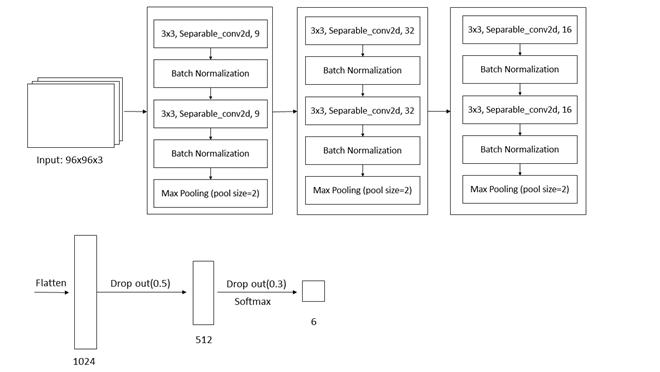
\includegraphics[width=\linewidth]{images/Quanh/ktmang.png}
    \caption{Minh họa kiến trúc mạng đã xây dựng}
    \label{fig:kientrucmang}
\end{figure}
% QUanhh viết r nè
% Do chip nhúng gì đó chỉ có bao nhiêu ram đó nên chúng tôi không thể xây dựng mô hình với trong số quá lớn và có chi phí tính toán cao được, nên chúng tôi sử dụng ...(thêm đoạn sau vô nè)
% Thêm dụ giảm kích thước của hình ảnh từ bao nhiêu đó xuống 96 * 96 nữa nà

Do sử dụng microcontroller cụ thể là board ESP32 camera AI Thinker, nên ram hỗ trợ rất khiêm tốn chỉ có 4MB. 

Nên chúng tôi không thể xây dựng mô hình với trọng số quá lớn và có chi phí tính toán cao. Khó khăn lớn nhất mà chúng tôi gặp phải khi xác định kiến trúc mạng CNN là không có một công thức cụ thể nào để tính toán dung lượng ram mà thiết bị sẽ dành cho lưu trữ và tính toán model.

Chúng tôi đã phải tiến hành nhiều thử nghiệm với nguyên tắc thử sai để tìm ra kiến trúc mạng tối ưu có thể dung hòa được hai yếu tố: đáp ứng giới hạn xử lý của thiết bị và hiệu suất phân lớp. Model CNN thường có khả năng phân lớp tốt trong trường hợp kiến trúc mạng có kích thướt lớn với nhiều tham số nhưng như vậy, sẽ quá khả năng xử lý của thiết bị. Ngược lại, nếu kiến trúc mạng có quá ít tham số, sẽ không đủ năng lực phân lớp ảnh để đáp ứng yêu cầu của bài toán.



Vì thế, chúng tôi chọn các sử dụng separable convolution thay cho lớp convolution thông thường để giảm bớt chi phí tính toán cho mạng. Ngoài ra ở lớp này, chúng tôi dùng regularization l2 để tránh overfitting và hàm kích hoạt relu – đây là hàm thường được sử dụng trong quá trình train model với dữ liệu dưới dạng ảnh. Chúng tôi cũng thêm các lớp batch normalization và drop out để tránh cho mô hình bị overfitting và loại bỏ sự kết nối chặt chẽ giữa các lớp fully connected. Tổng số tham số của mô hình là 532,161. Sau khi xây dụng mô hình, nhóm đã sử dụng optimization stochastic gradient descent với learning rate = 1e-4 và momentum = 0.8 để train mô hình. Cùng với việc giảm kích thước hình ảnh từ 512 × 384 pixels xuống còn 96x96 pixels để phù hợp với kích thước ram mà board hỗ trợ. Kiến trúc mạng cuối cùng được minh họa trong hình \ref{fig:kientrucmang}.

\subsection{Dataset và quá trình huấn luyện} % Giới thiệu về dataset ddùng để train và test 
% Dữ liệu được lấy từ cái gì đó quên oy, nhưng cái này nên thêm vô nha
% Kích thước của hình là ... không nhớ a
%The pictures were taken by placing the object on a white posterboard and using sunlight and/or room lighting. The pictures have been resized down to 512 x 384, which can be changed in data/constants.py (resizing them involves going through step 1 in usage).


Chúng tôi dùng bộ dataset TrashNet \cite{trashnet} của nhóm tác giả Gary Thung và Mindy Yang đến từ đại học StandFord để train và test model. Bộ dataset gồm 2527 hình thuộc 6 lớp, mỗi ảnh được chụp với ánh sáng mặt trời, một số ảnh còn có thêm ánh sáng phòng, vật được đặt trên nền trên giấy bìa trắng(láng). Ảnh sau khi chụp sẽ được resize xuống còn 512x318 pixels, số lượng ảnh trong mỗi lớp được phân bổ như sau:
 
\begin{itemize}
    \item Cardboard: 403
    \item Glass: 501
    \item Metal: 410
    \item Paper: 594
    \item Plastic: 482
    \item Trash: 137
\end{itemize}

Dữ liệu được chia làm 2 phần theo tỉ lệ 80\% train (2024 ảnh) và 20\% test (503 ảnh).

Sau đây là hình ảnh minh họa của 6 lớp cần phân loại như trên, được hiển thị ở bảng \ref{fig:trash_classification}.
\begin{table}[H]
    \centering
    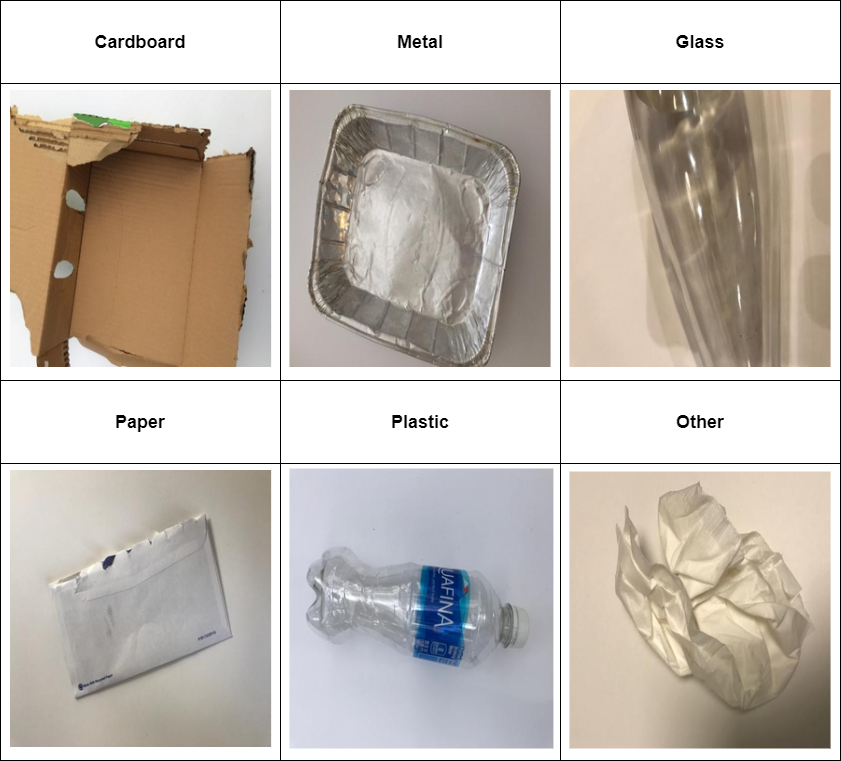
\includegraphics[width=\linewidth]{images/Quanh/Trash Classification.png}
    \caption{Phân loại hình ảnh trong bộ dataset}
    \label{fig:trash_classification}
\end{table}
% Nên lựa vài hình về data để thêm vô (nếu cần) hình nên có đủ 6 lớp cần phân loại
\subsection{Đánh giá hiệu quả của mạng CNN đã huấn luyện}

\subsubsection{Giới thiệu các độ đo tính hiệu quả của mạng CNN} % Các chỉ số để dánh gia model  %accuracy, F-score - Recall.
Chúng tôi sử dụng hai chỉ số là accuracy và F1-score để đánh giá model. Accuracy là tính tỉ lệ giữa số ảnh được dự đoán đúng và tổng số ảnh trong tập dữ liệu kiểm thử.

$Accuracy = \frac{TP+TN}{TP+TN+FP+FN}$

$Precision = \frac{TP}{TP+FP}$

$Recall = \frac{TP}{TP+FN}$

$F1 = \frac{2*Precision*Recall}  
{Precision+Recall} = \frac{2*TP}{2*TP+FP+FN}$
% Còn khúc giới thiệu F1 nữa cơ mà đang lười ghi công thức toán trong đây nha
% Khúc này thêm lý thuyết của hai cái chỉ số đó
\subsubsection{Kết quả  hiện thực được } % Kết quả  hiện thực được 
Kết quả train mô hình với 80 epoch
\begin{figure}[H]
    \centering
    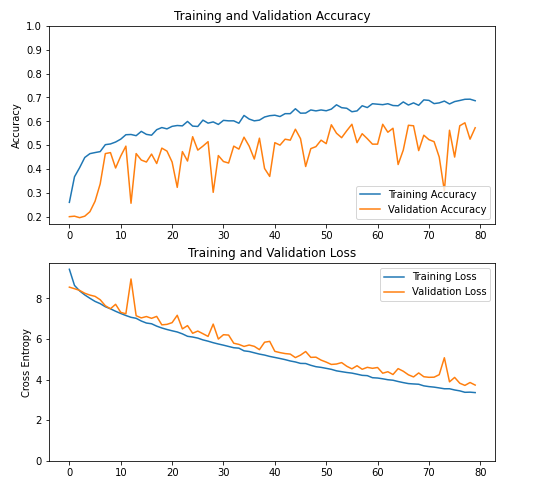
\includegraphics[width=\linewidth]{images/Quanh/graph.png}
    \caption{ Biểu đồ thể hiện loss và accuracy của mô hình trong quá trình train}
    \label{fig:graph}
\end{figure}
% Hai cái này nên chuyển thành dạng bảng, cơ mà đang lười chuyển
Accuracy cao nhất trên tập train là 0.6938 và trên tập test là 0.5938
Loss nhỏ nhất trên tập train là 3.3844 và trên tập test là 3.7116

Kết quả thử nghiệm mô hình trên tập test sau khi đã lưu mô hình tốt nhất từ quá trình train 
\begin{table}[H]
    \centering
    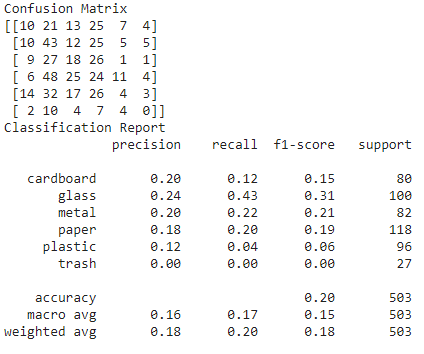
\includegraphics[width=\linewidth]{images/Quanh/matrix.png}
    \caption{Confusion matrix của model khi thử lại trên tập test}
    \label{fig:matrix}
\end{table}
Từ bảng \ref{fig:matrix} ta có thể thấy accuracy và f1-score của mô hình còn khá thấp, tuy nhiên do mô hình được xây dựng chỉ có 532,161 tham số nên không đủ để phân loại chính xác các lớp được. Chúng tôi đã thử train thêm epoch nhưng mô hình dễ bị overfitting và kết quả khi in confusion matrix vẫn không thay đổi nhiều. Ngoài ra nếu tăng thêm trọng số thì không thể sử dụng model trên thiết bị. 

Tuy nhiên, quay lại bài toán đã đặt ra, chúng tôi sẽ phân loại rác thành 2 lớp tái chế và không tái chế tương ứng với cardboard, glass, metal, plastic thuộc lớp tái chế và paper, trash thuộc lớp không tái chế. Như thế, chúng tôi thiết lập lại một confusion matix mới như bảng \ref{tab.newCM}. Từ đây, chúng tôi có thể tính được hiệu suất phân lớp của mô hình phân lớp ảnh rác thành hai lớp recycle và Non-recycle.

\begin{itemize}
    \item recycle presicion: 68.9%
    \item recycle recall: 67.87%
    \item recycle f1 score: 68.35%
    \item accuracy: 55.27%
\end{itemize}

\begin{table}[H]
    \caption{Confusion matrix đối với recycle và Non-recycle} 
    \label{tab.newCM}
    \centering
    \begin{tabular}{|l|l|l|}
        \hline
                & Recycle & Non-recycle\\ \hline
        Recycle & 243 & 115 \\ \hline
        Non-Recycle & 110 & 35 \\ \hline
    \end{tabular}
\end{table}



\section{Triển khai và kiểm thử mạng CNN phân loại rác trên thiết bị}
Sau khi model đã được train và evaluate kỹ lưỡng trên máy tính, công đoạn tiếp theo là build chương trình phân loại rác trên thiết bị dựa model đã train và thư viện TensorflowLite. 
Chương tình được build sẽ phải được kiểm thử để đảm bảo khả năng phân loại rác tương đương với khả năng phân loại của model đã được train trên ảnh từ PC.

\subsection{Quy trình triển khai code phân loại rác trên thiết bị}
%Mô tả lại quy trình chuyển đổi từ file h5 của model sang file .cc để đưa vào code
%Đưa vào các đoạn code mẫu của tensorflowLite
Sau khi đã hoàn thành các quá trình huấn luyện và thu được mô hình mạng CNN từ TensorFlow, cần xây dựng 1 chương trình có thể sử dụng mạng CNN đó để phân loại ảnh. Yêu cầu đặt ra với chương trình là nó có khả năng đọc hiểu các tham số bên trong mạng CNN và thực hiện được các phép tính cần thiết trên những tham số này, để đưa ra được kết quả dự đoán.

Công cụ quan trọng để cài đặt chương trình này là TensorFlow Lite. TensorFlow Lite là một thư viện mã nguồn mở về deep learning cho phép các models được huấn luyện bởi TensorFlow có thể chạy trên thiết bị. 

Đầu tiên, sau khi đã hoàn tất quá trình huấn luyện, chúng tôi sẽ sử dụng TFLiteCoverter trong TensorFlow để chuyển đổi model sang 1 định dạng có thể sử dụng được trong TensorflowLite. Bước chuyển đổi này cũng sẽ thực hiện một số thao tác tối ưu hóa (optimization) về mặt toán học với hy vọng có thể làm giảm yêu cầu tính toán và kích thước của model. Nhờ đó, phần nào giúp cho việc sử dụng model trên thiết bị dễ dàng hơn.  

Tiếp đến, chúng tôi sử dụng lệnh xxd của Linux để chuyển đổi file TFLite thành một mảng số ở dạng hexa nhằm mục đích có thể đưa vào sử dụng trong mã nguồn C++.  

\subsection{Quy trình thử nghiệm trên thiết bị}

%Đưa vào 2 đoạn code C++ và python và mô tả quy trình chạy:
%1. thiết bị start và chờ tín hiệu "bắt đầu chụp ảnh" từ code python trên PC
%2. Mình bấm 1 nút trên PC, code python sẽ gửi tín hiệu "bắt đầu chụp ảnh" qua thiết bị
%3. thiết bị chụp ảnh, lưu vào framebuffer của thư viện ESPCam rồi gửi qua cho code Python sau đó chờ tín hiệu "bắt đầu phân loại".
%4. Code python lưu ảnh xuống để thử nghiệm và sau đó gửi tín hiệu "bắt đầu phân loại" cho thiết bị.
%5. thiết bị chạy đoạn code phân loại rác của tensorflowLite và gửi kết quả cho code Python sau đó quay lại chờ tín hiệu "bắt đầu chụp ảnh"
%6. Code python hiển thị kết quả phân loại ra cho mình kiểm tra sau đó lưu lại, chờ người dùng nhấn enter để bắt đầu lại quy trình kiểm tra

Sau khi đã triển khai model vào thiết bị vào TensorflowLite, chúng tôi cần thực hiện thêm một bước kiểm tra để đảm bảo quá trình chuyển đổi và triển khai từ TensorFlow sang TensorflowLite không làm thay đổi đáng kể đến khả năng dự đoán của model.

Để thực hiện việc kiểm tra thiết bị ESP32Cam AI Thinker, chúng tôi đã viết một số chương trình python chạy trên laptop kết nối với thiết bị thông qua cáp micro USB. Mục đích của những chương trình này là để tương tác và nhận kết quả phân lớp ảnh từ thiết bị.

Chương trình python đầu tiên có chức năng kiểm tra kết quả phân lớp ảnh của thiết bị đối với những ảnh trong dataset \cite{trashnet}. Những ảnh này đã được huấn luyện trên model TensorFlow. Yêu cầu đặt ra là thiết bị phải có kết quả chính xác hoàn toàn với model được huấn luyện trên TensorFlow.

Chương trình python sẽ lần lượt đọc các ảnh trong dataset, sau đó tiến hành resize và truyền qua cho thiết bị tiến hành phân lớp. Sau đó đôí chiếu kết quả phân lớp của thiết bị với kết qủa phân lớp của model được huấn luyện trên TensorFlow. Và báo cáo nếu có sự khác biệt.

Chương trình python thứ hai có công dụng kiểm tra kết quả phân lớp của thiết bị đối với những ảnh mà chính camera của thiết bị chụp được. Việc kiểm thử này phải đáp ứng được gần đúng với yêu cầu mà mô hình thực tế hình \ref{fig:chart_smartbin}. Quy trình thực hiện viêc kiểm tra sẽ bao gồm các bước sau:

Khi nạp chương trình C vào board thành công qua cáp micro USB. Tắt chương trình C để nhường đường truyền cho chương trình kiểm thử trên python.

Để thay thế yêu cầu, khi ultrasonic sensor gặp vật cản sau đó khởi động chụp ảnh, thì trong môi trường kiểm tra. Chúng tôi dùng một input được nhập từ bàn phím (nhấn enter) để thay thế bước trên. 
\begin{enumerate}
    \item Nhận input từ người dùng: khi nhấn enter: 
    \item send "1" đến board.
    \item nhận hình và kết quả dự đoán từ board .
    \item save hình vào local (cùng thư mục vs python, tên file là thời điểm nhận hình).
    \item show kết quả dự đoán trên console và bật app show ảnh ( đã save ở 4)
\end{enumerate}

\subsection{Kết quả phân loại khi chạy trên thiết bị}

%Đưa vào vài tấm hình được thiết bị chụp và kết quả phân loại tương ứng. 
%Sau đó chém gió là thiết bị chạy ra kết quả y chang như model đạt được ở mục trước
Một số hình ảnh được chụp từ thiết bị:
\begin{table}[H]
    \centering
    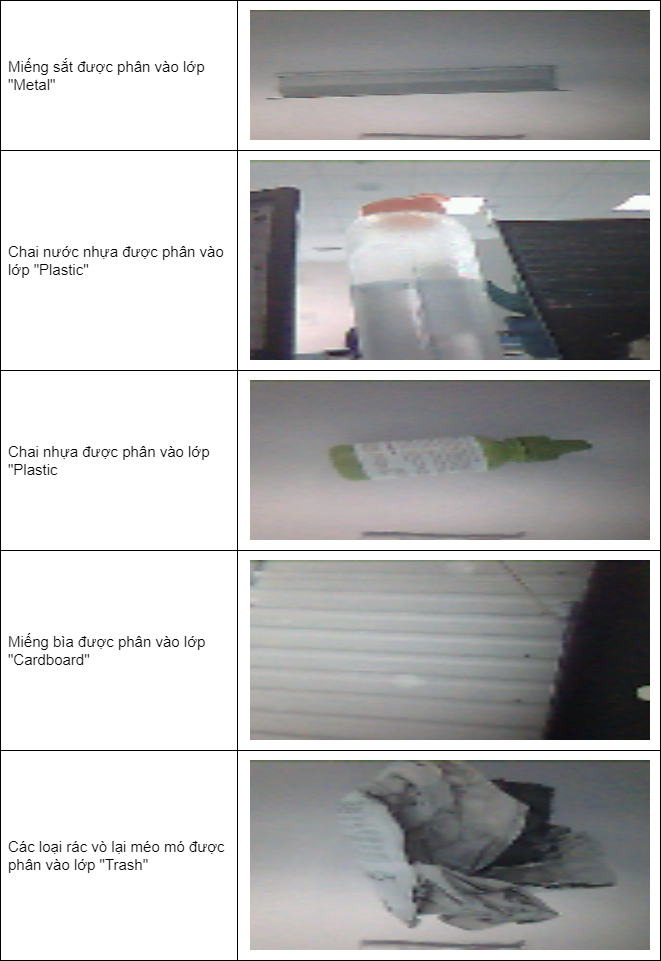
\includegraphics[width=\linewidth]{images/Quanh/Trash Result.png}
    \caption{Kết quả phân loại của một số hình ảnh}
    \label{fig:trash_result}
\end{table}

Tuy nhiên, do accuracy của model chỉ ở mức tương đối, và hình ảnh được train và hình ảnh được chụp từ thiết bị sẽ có thay đổi về màu sắc. Nên sẽ có một số loại rác bị detect sai. Dưới đây là các trường hợp sai trong quá trình kiểm thử.
\begin{table}[H]
    \centering
    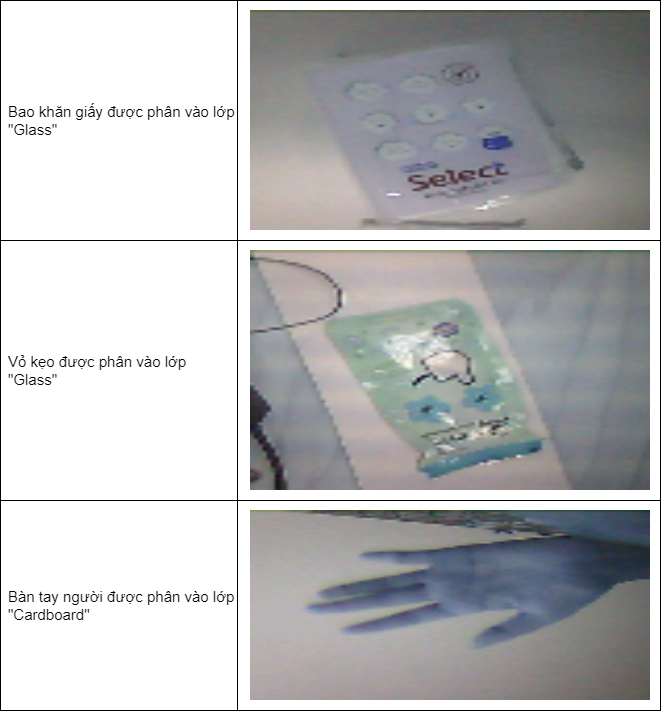
\includegraphics[width=\linewidth]{images/Quanh/Trash Failed.png}
    \caption{Một số kết quả sai trong quá trình phân loại}
    \label{fig:DWglass}
\end{table}

Như vậy, tuy có các trường hợp detect sai, nhưng có thể hình dung được mức độ đánh giá của model trong việc detect hình ảnh. Ví dụ như ở bảng \ref{fig:DWglass}, mặc dù đã bị detect sai lớp, nhưng có thể thấy, thủy tinh nói chung đều có tính chất phản ánh sáng, nên khi hình ảnh khi chụp 1 vật làm bằng thủy tinh sẽ có một độ bóng nhất định. Vì thế ở 2 hình đầu  đều có tính chất phản ánh sáng như thủy tinh, nên thiết bị sẽ detect vào lớp "glass". Tương tự, các miếng bìa hầu hết trong tập dataset đều có các lằng vân nhấp nhô, và khi thiết bị chụp hình ảnh bàn tay người, bàn tay cũng có các đường chỉ tay sâu, nên thiết bị sẽ detect vào lớp "cardboard".

\section{Setup Gateway}
\subsection{Access LG02}
Cấp nguồn điện cho gateway, sau đó dùng laptop để bật scan wifi, lúc này sẽ xuất hiện tên wifi : “dragino-168cb0”

Kết nối với wifi đó và truy cập địa chỉ IP: “10.130.1.1”, lúc này sẽ đến giao diện để configure gateway bằng cách nhập username và password như hình \ref{fig:gateway_configure}
\begin{figure}[H]
    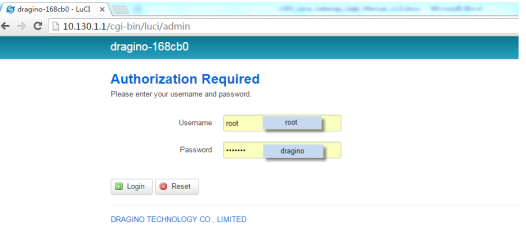
\includegraphics[width=\textwidth]{images/Quanh/Gateway_configure.png}
    \caption{Xác thực tại địa chỉ 10.130.1.1}
    \label{fig:gateway_configure}
\end{figure}

\subsection{Cài đặt network}
Truy cập Internet như Wifi Client theo các bước:
\begin{description}
    \item Bước 1: Network → Wireless, chọn radio0 và scan như hình \ref{fig:radio0_scan}
    \begin{figure}[H]
        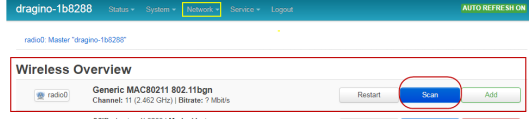
\includegraphics[width=\textwidth]{images/Quanh/Radio_scan.png}
        \caption{Scan mạng Wireless}
        \label{fig:radio0_scan}
    \end{figure}
    
    \item Bước 2: Chọn wifi và tham gia vào mạng, sau đó nhập mật khẩu và Submit như hình \ref{fig:join_password}
    \begin{figure}[H]
        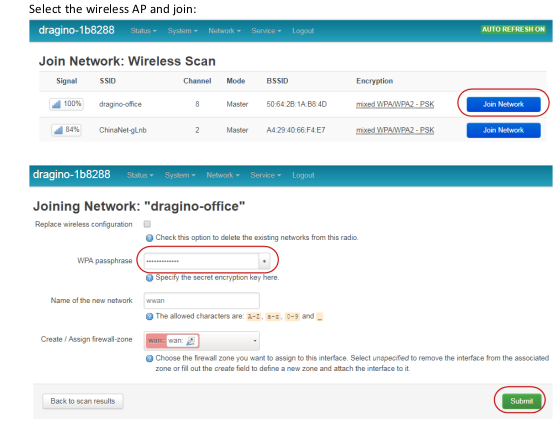
\includegraphics[width=\textwidth]{images/Quanh/Join_password.png}
        \caption{Tham gia vào wifi và nhập mật khẩu}
        \label{fig:join_password}
    \end{figure}
    \item Bước 3: Network → Wireless, chọn disable wifi mặc định của gateway như hình \ref{fig:disable_wifi}
    \begin{figure}[H]
        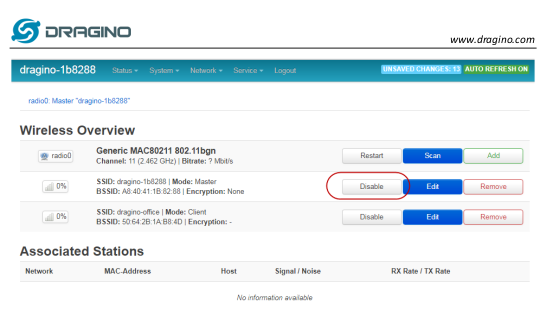
\includegraphics[width=\textwidth]{images/Quanh/Disable_wifi.png}
        \caption{Tắt wifi mặc định}
        \label{fig:disable_wifi}
    \end{figure}
\end{description}
(lưu ý, sau khi thực hiện bước 3, kết nối sẽ bị mất, nếu laptop kết nối wifi mặc định lúc nãy)

Trong trường hợp không thể truy cập địa chỉ 10.130.1.1 nữa, ta sử dụng cổng LAN để kết nối:
\begin{enumerate}
    \item Kết nối LAN Port
    \item Configure Ethernet port có địa chỉ IP là 172.31.255.253 và network 255.255.255.252.
    \item Dùng địa chỉ 172.31.255.254 để truy cập vào Web
\end{enumerate}


\subsection{Tạo gateway trên TTN Server}
\begin{description}
    \item Bước 1: Vào Service → LoRa → Lấy ID của Gateway như hình \ref{fig:get_gateway_id}
    \begin{figure}[H]
        \centering
        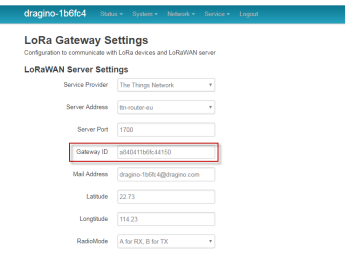
\includegraphics[width=\textwidth]{images/Quanh/Gateway_ID.png}
        \caption{Lấy ID của Gateway}
        \label{fig:get_gateway_id}
    \end{figure}
    \item Bước 2: Truy cập TTN: https://console.thethingsnetwork.org/gateways, giao diện hiển thị ở hình \ref{fig:gateway_console}
    \begin{figure}[H]
        \centering
        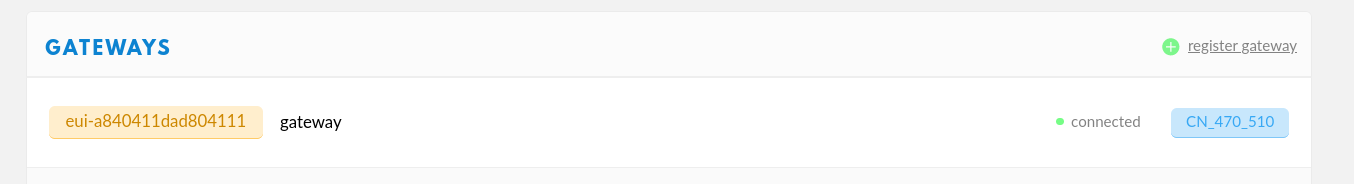
\includegraphics[width=\textwidth]{images/Quanh/Gateway_console.png}
        \caption{Giao diện Gateway đã được tạo (chưa connect)}
        \label{fig:gateway_console}
    \end{figure}
    \item Bước 3: Nhập ID vào Frequency plan tùy thuộc vào Gateway mà chọn cho phù hợp như hình \ref{fig:choose_gateway}, và kết quả status hiển thị là sẽ hiện "connected".
    \begin{figure}[H]
        \centering
        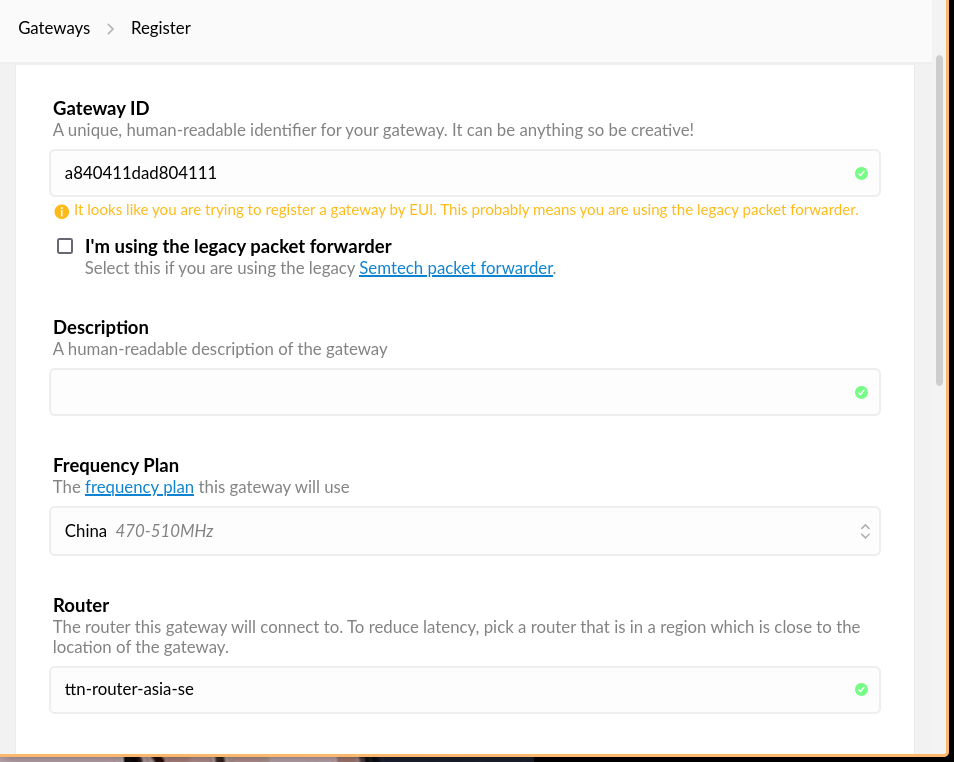
\includegraphics[width=\textwidth]{images/Quanh/Gateway_choose.png}
        \caption{Nhập ID vào Frequency plan}
        \label{fig:choose_gateway}
    \end{figure}
\end{description}
**do Gateway của nhóm sử dụng frequency 433Mhz nhưng The Things Network không hỗ trợ nên khi đăng kí sẽ là : china 470-510Mhz ( do tần số 433 trãi từng tần số 433 đến 510)

\subsection{Configure LG02 Gateway}
\begin{enumerate}
    \item Configure to LoRaWAN server qua các bước:
    \begin{description}
        \item Bước 1: Config LG02 với IoT Service là Lorawan/RAW forwarder, sau đó Save \& Apply
        \item Bước 2: Chọn Service Provider là The Things Network, Server Address là ttn-router-asia-se và Server Port là 1700
    \end{description}

    \item Configure LG02's RX frequency: Ở frequency 433Mhz, có 8 channel uplink nhưng nhóm chọn channel 433.175Mhz để end-device join vào, thông sô như hình \ref{fig:radio_config}
    \begin{figure}[H]
        \centering
        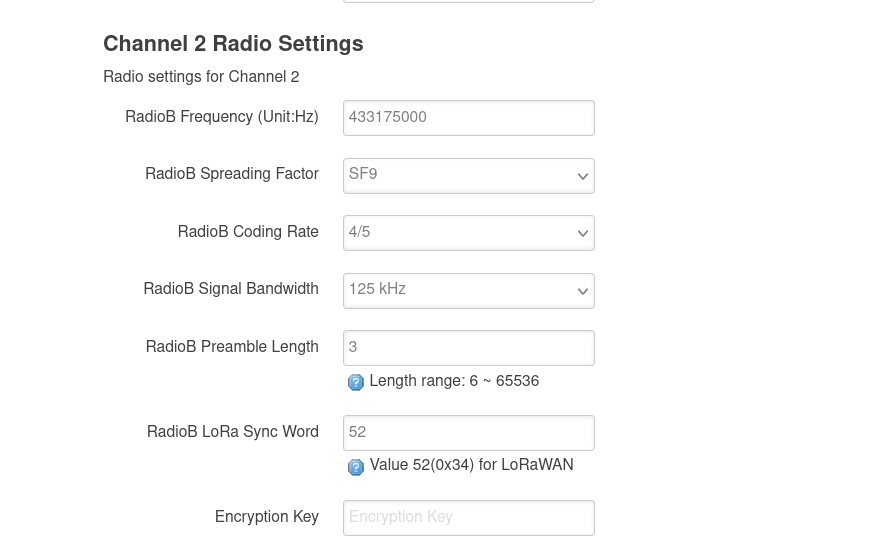
\includegraphics[width=\textwidth]{images/Quanh/Radio_config.png}
        \caption{Thông số configure}
        \label{fig:radio_config}
    \end{figure}
\end{enumerate}


\section{Setup End-Device}
\subsection{Thu gom rác}
Phần mềm sử dụng: Arduino IDE 1.8.2

Ngôn ngữ lập trình: C

Thiết bị Kit RF thu phát wifi Blue esp32 + Lora sx1278 oled Heltec.

\begin{description}
    \item Bước 1: Add lib esp32 từ link https://github.com/HelTecAutomation/Heltec\_ESP32 để thêm thư viện esp32 cho Arduino
    \item Bước 2: Add lib Lmic https://github.com/matthijskooijman/arduino-lmic để thêm vào thư viện Lmic cho Arduino
\end{description}

** Thư viện esp32 hỗ trợ hoạt động trên Heltech ESP32 develop framework.
** Thư viện Lmic cung cấp các giao tiếp LoRaWan ở classA và Class B. Tuy nhiên chỉ hỗ trợ ở band EU-868 và US 915. Nhưng thiết bị nhóm sử dụng là frequency 433Mhz nên cần sửa 1 số file để thiết bị có thể truyền data

Lúc này, có thể nạp code vào board như bình thường.

\subsection{Đăng kí trên TTN Server}
\begin{description}
    \item Bước 1: Tạo Application ID và handler, sau đó vào Devices → Register device → Điền Device ID  
    \item Bước 2: Sau khi đăng kí device thành công, The Things Network sẽ mặc định setup device join vào channel theo OTAA, nhưng nhóm chọn join theo ABP nên cần vào Setting → Activation method → ABP.
    
\end{description}



** ở phần này Payload Formats sẽ tùy thuộc vào code nạp vào end-device



\subsection{So sánh khi sử dụng Cayenne LPP và Custom}

Ta có bảng \ref{tab.comparison.Cayenne}

\begin{table}[H]
    \centering
    \caption{Loại rác} 
    \label{tab.comparison.Cayenne}
    \begin{tabular}{| m{6cm} | m{6cm} |}
        \hline
        Cayenne LLP & Custom \\

        \hline
        •	Không cần decoder (do thư viện Cayenne LPP đã có những quy định về code ở end-device) & •	Cần decoder để TTN hiển thị thông tin \\
        •	Khó hiển thị thêm các trường data từ sensor khác (Vì chỉ  hỗ trợ mặc định cho sensor nhiệt độ độ ẩm, các sensor khác phải qua pin Analog) & •	Có thể thêm nhiều sensor dễ dàng bằng code trên node, và chỉ cần cài đặt Payload formats trên TTN để hiển thị thông tin \\
        •	Mặc định payload & •	Có thể thay đổi Payload \\
        
        \hline
    \end{tabular}
\end{table}

Để chuyển data cho backend, cần cấu hình ở phần Integrations.



\subsection{Lưu ý khi nạp code cho node}

Vì sử dụng phương thức join vào server là ABP nên cần khai báo các thông tin cần thiết vào file *.ino để node có thể send data đến application server 

\begin{itemize}
    \item Device EUI, Network Session key và App Session key
    \item Để tối ưu việc truyền nhận từ node đến gateway,  nên disable các channels không cần thiết( chỉ enable channel đã khai báo ở RX của gateway)
\end{itemize}



